\chapter{Detection and Integration}
\label{chap3}

\section{Preface}
The major problem faced during this work is related
to the detection of intruders while surveilling the house.
Modern security systems applies different techniques to detect intrusions
using many different sensors such as leap motion detection, face detection
or sound analysis. They have been working fine during the last years, however
thieves improves bypassing or partially avoiding these technique making the latter
less effective.\\
Therefore most of the work will be done investigating and testing innovative and
advanced techniques to deal with intrusions detection.

\section{Fingerprinting a Human}

During the time there has been many approaches to recognize a "Person"
using some of its peculiarities: software side with passwords or access phrases,
which should identify a single person; biometrics with finger prints, retina scans
and voice recognition.\\
Usually such controls where available only with expensive solutions (and some still are, e.g. retina
scanners), however with the introduction of \textit{IoT} their price dropped allowing
them to be sold for a reasonable price. These controls are also called \textit{behavioral biometrics},
the set of behavioral traits which identifies an individual person. Usually these traits are
used for authentication when accessing a restricted system, however we'll consider
these to recognize unknown entities accessing our house. \\
These systems are mainly needed to prevent accidental triggering of the alarm, to be more
precise when listening or watching, not detecting just something but a real intrusion.

\subsection{Behavioral biometrics}
Detecting if someone in the house is someone familiar is not an easy task, most
of the approaches are precise in optimal conditions, much less when the situation
is non optimal (low light, low resolution etc). This impacts negatively their efficiency
when applied in a real life scenario, where usually the conditions are far from the optimal
situation. For example facial recognition works in very limited cases, like the systems
used on smartphones to unlock the device, has been reported to not be reliable enough
to be the main unlocking system. The situation is also similar for voice recognition or
speech to text systems, which are improving during the time and mainly \textit{during the usage}.
\textit{Siri}, one of the most famous personal assistant had some minor troubles at the beginning
being used to the different users voices, accents and languages. \textit{Siri} uses
different voice recognition algorithms to categorize your voice by learning your
dictation and your accent, with better results over time.


\section{In House Speaker Recognition}

A house is an ideal place where to place a speaker recognition system,
since there are not many noise sources, ensuring a good quality input
for microphones. Hence a good surveillance system with many microphones around
the house should be able to detect any external voice during an intrusion. In the following
paragraphs we'll show how we implemented such a system using some of the state-of-the art
algorithm with \textit{Calvin} to improve the security in the house.

\subsection{Speaker recognition and Calvin}

Machine learning tasks are typically cpu and time consuming tasks, which
are not supposed to run on low-resource machines like a Raspberry Pi. However
we need to access physically some sensors to gather the input and not many computers
offer direct GPIO access, making devices like a Raspberry Pi a must when interfacing
with hardware. Despite of this limitation \textit{Calvin} offers the solution to this problem
when adopting the philosophy of \textit{"run it where you need"}. As said in the previous chapter
Calvin actors can run on different machines, and communicate through the network.
As can be seen in figure \ref{fig:calvin-spkr1}, in the basic configuration we need two machines:
one interfacing with the hardware, mainly a microphone and a sound detector, and a more powerful
machine.

\begin{figure}[h]
\caption{Spaker Recognition Architecture with Calvin}
\label{fig:calvin-spkr1}
\centering
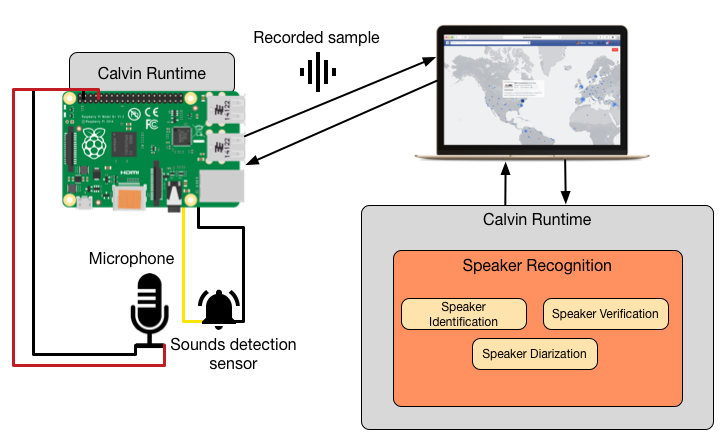
\includegraphics[scale=0.50]{calvin-speaker1.png}
\end{figure}

In more detail, in our architecture there will be 2 actors controlling the input from
the two sensors, and at least 3 in the other machine, each of them taking care of a different
task, namely identification, diarization and verification.

\subsection{Actor Structure and Interaction}

The interaction between actors in this situation can be summarized as a chain
of events triggered by the detection of a sound to the detection of a person, either
familiar or unknown. In our proposed architecture an Actor linked to the sound detector sensor
will continue listening, and when something is detected it will generate a token for the microphone Actor
to switch to the recording state for a finite period of time. However it is not possible to stream in real time the recording
to another machine without overcomplicating the system, for which we proposed to split the original
audio recording in small pieces to be sent through the network. This approach has some theoretical benefits:

\begin{itemize}
    \item Dividing the record in small units make it faster to detect someone, since the
    verification phase will require less time.
    \item Small audio recorded files are easier to send instead of a single big one.
\end{itemize}

Despite of the benefits, in the following chapter we will try to prove the effectiveness of this approach,
and the best duration of time for each time slot.\newline
After recording the audio slice the Actor will have to send it to the identification /diarization/ verification
actor residing on a different machine. However sending binary objects through the network
may be tricky without working directly with sockets, in our solution we decided to
use the \textit{base64} encoding and envelope it into a JSON object. The object will be decoded
and stored as a binary object and subsequently the machine learning actor will execute
its algorithm on it.

\subsection{Hardware Interacting Actors}

In this section we'll go into the details of the low level actors handling the resources
such as sound detection and microphone, describing their internal logic and actions.

\subsubsection{Sound Detection Actor}

The simplest actor is the one dealing with the sound detection. It's state works
as a simple switch turned on by the change of state of the sensors. This actor does
accept only an input, the trigger for reading the sensor value. This allows us to
decide at which rate reading the sensor without leaving the read rate to the internal
scheduler. The actor generates only a token each time the value read by the
sensor is equal to 1 (i.e. a sound is detected). Therefore the conditions
of the Actor can be seen in listing \ref{cond1}.

\begin{lstlisting}[language=Haskell,frame=single,caption=Sound Actor conditions,label=cond1]
    Condition for receiving the input
    @condition(action_input=['trigger'])

    Condition for returning the output
    @condition(action_output=['token'])

\end{lstlisting}

 The conditions shown in figure \ref{cond1} will bound the input and outputs to the correct functions.
 Furthermore, to clarify the internal state change of the actor here is shown
 how the control on the sensor reading using the \textit{Calvin} \texttt{@guard}
 statement:
 \begin{verbatim}
     @guard(lambda self: self['sensor'].read_state() == 1 and self.trigger)
 \end{verbatim}
 The sensor can be accessed through a managed object handled by the \textit{calvinsys}
 layer, hiding the implementation details. Moreover the \texttt{self.trigger} secondary
 condition requires the Actor to be in possession of a valid token, which will be consumed
 after each reading.

 \subsubsection{Recording Actor}

 The recording actor will have some more complicated logic having to deal with
 the audio sampling. The Actor will be bounded to the former actor to receive
 the token and start the recording process. As said previously we decided to
 take a different approach, instead of a single recording we will sample it in
 $n$ segments of the same duration. The Actor will therefore change its state
 in order to generate the needed amount of audio recordings to be sent to the
 speaker recognition Actor(s).\newline
 In figure \ref{cond2} can be seen the many conditions applied to the actor in order to fire the many actions.

 \begin{lstlisting}[language=Haskell,frame=single,caption=Sound Actor conditions,label=cond2]
 Initialize the actor with a number of samples and their duration
 @manage(['n_samples','duration'])
 This is a one time initialization, without bounding
 these parameters to any inbound port.

 The condition for setting the actor as active, coming from the
 sound detector
 @condition(action_input['token'])

 The outbound connection is a bas64 encoded audio recording
 loaded into a json object
 @condition(action_output['wav'])
 \end{lstlisting}

 However the former skeleton doesn't explain enough about the internal structure of the Actor,
 for which the more specific guard conditions explains it in more detail.\newline
 The guard condition in figure \ref{cond6} starts the recording process of an audio sample,
 with three conditions to match:token available, the number of recordings done and the microphone state.
 \begin{lstlisting}[language=Haskell,frame=single,caption=Sound Actor conditions,label=cond6]
 @guard(lambda self: self.token and
    self.token_used > 0 and not self['microphone'].recording())
 \end{lstlisting}
\pagebreak
 It is necessary to clarify the behavior of some internal variables:

 \begin{itemize}
     \item token - is a variable set to True each time a token is received from the previous
     actor. It gets voided when the actor dispatches all the $n$ audio recordings.
     \item token\_used - an internal variable initialized to $n$ each time the actor receives
     a token and decremented each time the actor sends an audio file to the speaker recognition actor.
     \item wav - is a simple flag representing the availability of a wav file to dispatch
     \item microphone - is the physical sensor managed from the \textit{calvinsys} layer.
 \end{itemize}

\subsection{Speaker Recognition Actors}

In this section we will go further with the Actors specialized
in the \textit{Speaker Recognition} task, namely: Speaker identification
and speaker diarization.

\subsubsection{Speaker Diarization}

As introduced in the previous chapter, speaker diarization is the process of
finding the various speakers in an audio recording. The Actor supports only two
functions: extracting the speakers and adding models to use in the identification phase.
The diarization works in two phases: first the system splits the recording in many clusters
based on who is speaking, and subsequently it tries to identify the voices from the
models in the database.\newline
The Actor accepts the following inputs:
\begin{itemize}
    \item wav - The base64 encoded audio recording from an audio source (i.e. the former microphone actor)
    \item operation - The operation to perform on the file, either extracting speakers or adding a model to the database.
    \item model name - An unique identifier for the new model to be added in the database
\end{itemize}

Therefore the output connections will be:

\begin{itemize}
    \item number of matches - the number of different speakers in the audio recording
    \item matches - the models for which there was a positive match in the database, unknown otherwise.
\end{itemize}

The conditions in figure \ref{cond3} apply in order to maintain a proper flow in the execution.

\begin{lstlisting}[language=Haskell,frame=single,caption=Sound Actor conditions,label=cond3]
    These conditions only apply when receiving and returning
    values:
    @condition(action_input=['operation'])
    @condition(action_input=['wav'])
    @condition(action_input=['model_name'])
    @condition(action_output=['n_people','names'])

\end{lstlisting}

However these conditions don't express the real logic beneath the Actor, which
is handled by the \texttt{@guard} conditions. Here follows the most
important guard conditions.\newline

The guard shown in figure \ref{cond3} allows us to set the operation only when it's unset,
restricting the set of possible choices for the operation.

\begin{lstlisting}[language=Python,frame=single,caption=Sound Actor conditions,label=cond3]
    @guard(lambda self, operation: self.operation ==
        None and (operation == 'extract' or
        operation == 'add_model')
\end{lstlisting}

The guards conditions illustrated in figure \ref{cond4} are used for the two steps
asynchronous recognition. The first phase start the process
and needs some parameters to be set properly:
the operation must be extract, the wav file has to be set
and extracted means we did not pass already this phase.

\begin{lstlisting}[language=Python,frame=single,caption=Sound Actor conditions,label=cond4]
    @guard(lambda self: self.operation == 'extract' and self.wav
        is not None and not self.extracted
\end{lstlisting}


In conclusion, the Actor's purpose is to identify the different
speakers and if they match with someone in the database return
their names.

\subsubsection{Speaker Verification and Identification}

Due to the subtle difference between identification and verification, we have decided to encapsulate them
 in a single actor. Speaker Identification is applied when no
model to identify is given, meanwhile verification is executed when a model to match
is available. The structure of the Actor is very similar to the one proposed in the
previous: the actor accepts as input a wav file (base64 encoded) and a model name
(in this case is optional), and an operation parameter for adding models to the database.
Therefore the input are equal to the previous actor, though this time operation may
be only restricted to \textit{recognize} and \textit{add model}. However the outbound
connection of the Actor will be different, this time the actor will return the likelihood
of the match, and the model for which there was a match (if it is identification).



\section{Expanding the system}
One of the biggest limitations of nowadays security system is their isolation
when installed. Most of devices are stand alone solutions incapable of extending
their functionalities to pre existing devices. If we want to expand \textit{Calvin} to
be adopted by others, including users and developers, we need to be able to extend its
functionalities with the ability to communicate with different other systems.

\section{The Architecture}

In this section we will go deep in the details of the architecture of the solutions
we propose.

\subsection{Accessing different systems}

Accessing different systems is a problem of technology interoperability between
different technologies running on architecturally different hardwares.
Most of the times \textit{IoT} devices runs on low limited power devices such as
an \textit{Arduino} or a \textit{Raspberry Pi}, both supporting different system
languages (the first is limited to a subset of \textit{C++} meanwhile the second one supports everything
that can run under a normal linux distribution, but usually it's \textit{Python}).
However in our scenario the devices we consider are on a different layer of abstraction,
we do target ecosystems and not single independent devices. \textit{Ecosystems} has to
provide an access to developers through a point of access, \textit{REST api} for   \textit{Nest}
and the \textit{HomeKit.framework} for accessing \textit{HomeKit} devices.
The limitations are not always the same, when using \textit{Nest} it's easier to communicate
with it using a wrapper for their own api, which exists in many libraries, including \textit{Python}.
Nonetheless the situation with \textit{HomeKit} is much more strict, having their ecosystem
restricted only to their technology, \textit{Objective-C} or \textit{Swift}, which runs only
on \textit{Apple} branded device. Furthermore, the limitations are even more strict
due to the limitation of the framework only for \textit{iOS}, at the moment at least.
Usually the latter is the common case, which implies the need of a different solution
then "just wrapping" the apis in the code and plug them into the project.
In our case \textit{Calvin's} system is fully written in \textit{Python},
though it have many extension for a wide range of technologies, communicating
with \textit{HomeKit} is still hard to achieve.
In the following sections we'll describe the approaches taken to solve
the problem.


\section{Accessing Nest}

As said in the previous section \textit{Nest} has some advantages
due to their cloud apis, which makes it easier to reach the connected devices.

\subsection{Nest API Model}

\textit{Nest} offers a cloud API near real time, based on a subscription, that allows
users to build products accessing data on their devices, with the relative ability
to read and write data. With the \textit{Nest} cloud each element is identified as a resource
and accessible through a unique address, called "data location".
Furthermore, the cloud system also offers a \textit{RESTful} service to access these resources,
but only allowing GET and PUT operations with a call limit to prevent overuse. There is also
a \textit{Streaming} feature for REST, which allows our application to receive updates
in real-time or to stream from a device, namely camera, since web-sockets are not supported.
However it applies the same rule as before, with some limits in the data usage to prevent abuse.



\begin{figure}[h]
\caption{Nest Cloud architecture}
\label{fig:nestarch}
\centering
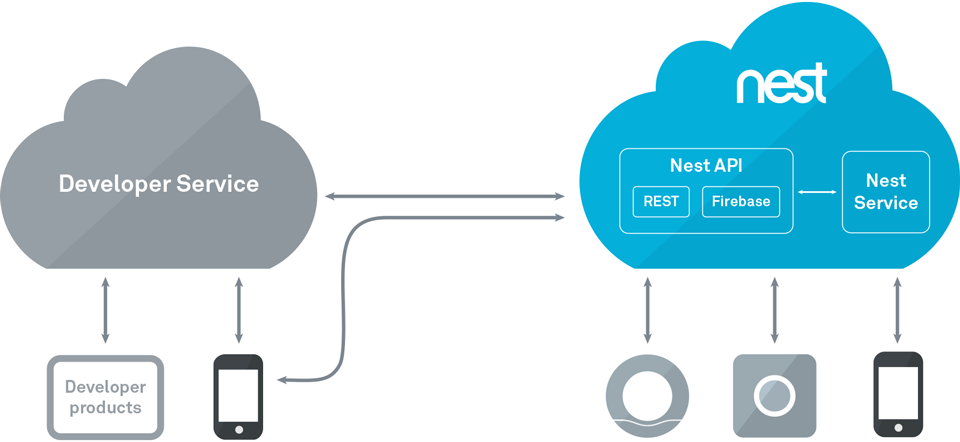
\includegraphics[scale=0.35]{nest-architecture.png}
\par{Source: Nest Inc}
\end{figure}

As can be seen in figure \ref{fig:nestarch}, the only way to access \textit{Nest} devices at the
moment is only through their cloud system. However this will add many layers of overhead
and delay due to the various layers, including calling services external to our network. However,
in the upcoming future it will be also possible to use \textit{Nest Wave}, a direct device
to device communication through protocols such as BLE or Wi-Fi, moving the integration to a higher
lever of quality.



The cloud functions of \textit{Nest} are limited to a restricted set of devices:
Thermostat, Protect (alarm), Camera and the Home.
Here are the functionalities offered by each of the products, with a brief description:
\subsubsection{Nest Thermostat}
Thermostat, as the name suggests, is a smart thermostat ,which can also be remotely controlled,
with some energy saving settings to help the user avoiding unnecessary heating expenses.   \\
Its remote functionalities are:

\begin{itemize}
    \item Read the current temperature
    \item Read or set a target temperature
    \item Set the fan timer
    \item Read or set the temperature mode
    \item See humidity values
    \item View online status and last connection information
    \item Read structure name and device location in the home
\end{itemize}

\subsubsection{Nest Protect}
Protect is a location based alarm for dangerous gas leaks, such as  Carbon monoxide \textit{CO}, or
smoke in case of fire.

\begin{itemize}
    \item View CO or smoke status
    \item View battery health state
    \item View online status and last connection information
    \item Structure name and device location in the home
\end{itemize}

\subsubsection{Nest Camera}
Camera, previously known as Dropcamera, is one of they key components of the
\textit{Nest} suite. It provides screen capture, audio and video streaming and the
other typical features offered by smart cameras.

\begin{itemize}
    \item View camera online status or mic status
    \item View or change streaming status (turn video streaming on/off)
    \item View device name and where identifier
    \item View content related to the last event that triggered a notification, including:
        \\Sound or motion event detected
        \\Event start/stop times
    \item Structure name and device location in the home

\end{itemize}



\subsection{Nest with Calvin}

One of the key aspects of \textit{Calvin's} Actors is their abstraction
to allow their reuse in different situations. However, due to the different
nature of the ecosystem, specially \textit{Nest} and \textit{HomeKit} the actors
can't be used for the same purpose.
\textit{Nest} structure can be decomposed in two big sections: Structures and Devices.
Structure are objects to keep grouped together many devices, placing them in different part of the house,
but still not the most important part in our scenario.\\
A device is an abstraction of all the smart products offered by Nest, but mainly the one we have listed in the latter
paragraph.

\subsubsection{Device Abstraction}

We have abstracted a device in its most basic functions: setting and getting properties.
This simplification allows us to follow the best practices for the development of \textit{Calvin},
allowing a possible reuse of the actor. Here is the pseudocode for the high-level functions definition.

\begin{verbatim}
    getproperty: in device_id, property_name; out property_value
    setproperty: in device_id, property_name, value ; out True or False
\end{verbatim}


However going deeper into the actor architecture we have to define some more constraints,
like the events which trigger the execution and the tokens for which returning the results.
All incoming port of an actor has to be linked, we can not have an unbounded port,
both input or output. Listing ~\ref{code2} shows an example of connection bounding for incoming
and out-coming connections.\pagebreak


\begin{lstlisting}[language=C,frame=single,caption=Example resource response,label=code2]
    Inputs:
        device: the device identifier
        operation: string representing
            the operation to do (get or set)
        property_name: the property to be get/set
        value: the value to be used to
            set the property
    Outputs:
        result: the property value
\end{lstlisting}

To simplify the work, we reduced the inbound port for the operation to only one, instead of having a token
for a \textit{get} or \textit{set} operation. This task is completed using the \texttt{@condition} to declare
all the elements which are needed to fire and will be used in a particular action.
A simple condition for an action is the following example:
\begin{verbatim}
    @condition(action_input=['operation'], action_output=[])
\end{verbatim}
This condition requires the token operation to be bounded, and it will use it in its body function. Since
no \texttt{action\_output} is defined, the operation does not return any value.

Once all the inbound ports are connected, i.e. they have a token, the system will check the \texttt{@guard} condition,
which acts as a conditional control: it will continue only if the condition is satisfied.
An example guard condition can be written as:

\begin{verbatim}
    @guard(lambda self: self.nest._in_progress is
        None and self.operation == "set")
\end{verbatim}
This guard condition is used to enter the function only when the \textit{nest} object is not
working on an asynchronous task and the operation has to be the \textit{set} operation.\\
One of the constraints that an actor has to follow is the \textit{reactivity}, which implies
non-blocking calls in the body of its functions. However, as in our case, the actor will have to
make some calls to the \textit{Nest} cloud, which is a blocking call. This is reached
using a two step asynchronous system: first the value is acquired and the actor
will delegate the request to a different thread; second when the delegate terminates it will
modify a flag to mark its completion, at that point the actor will return the value obtained
from the nest cloud. Asynchronous calls are needed since the scheduler loop can't be blocked
during the execution otherwise it would break the reactivity of the other actors.

\subsection{A Microservice Oriented approach}

Despite of the correctness of the former solution, it does however contains some
flaws in the architecture. The solution works only under the following circumstances:

\begin{enumerate}
    \item Libraries for connecting to a different ecosystem are provided in the same language (e.g. \textit{Python}).
    \item We assume the actor does never crash, and if it does the system may crash subsequently.
    \item The integration library won't require any change or modification in the future.
\end{enumerate}

However these assumptions are too risky to be considered for an always running system, because the likelihood
of one of the above problems to happen is very high.\\
To face these problems we adopted a \textit{microservice} architecture style to implement the integration with
other ecosystems. In the case of \textit{Nest} is not very significative but it will be much more for \textit{HomeKit}, as
we'll see later.

\subsubsection{Microservice Architecture}


\begin{figure}[h]
\caption{Microservice Integration architecture}
\label{fig:test-arch}
\centering
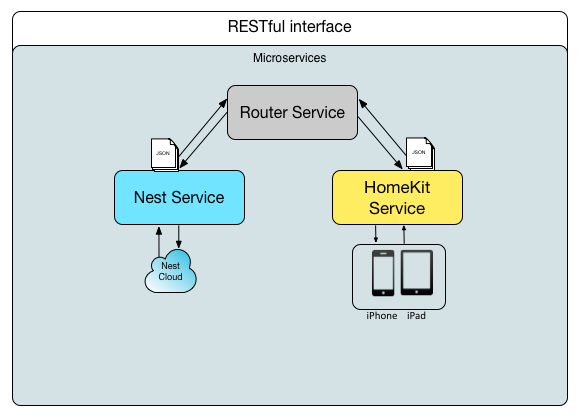
\includegraphics[scale=0.65]{test-arch.png}
\end{figure}

Figure \ref{fig:test-arch} illustrates the architecture proposed in our solution.
All the microservices can be reached through a router service, which doesn't expose
the real location of each service. This approach moves the service finding logic outside
of \textit{Calvin}, simplifying the work of the actor who won't have to deal with possible
re-deployments or re-locations of the service, it will just need to know where to reach the
routing service. This task will be deferred to the \textit{routing} service, which will act
as a proxy to the other micro-services.\\
Each ecosystem has a microservice dedicated, this is due to the different internal structure of the
different technologies. For example \textit{HomeKit} uses a hierarchical structure divided in the following,
from above to the bottom: \textit{HMHome}, \textit{HMRoom}, \textit{HMAccessory}, \textit{HMService} and \textit{HMCharacteristic}.
Which differs from the simpler one of \textit{Nest}, where there are mostly Structures and Devices.\\
Moreover structuring the integration with ecosystems introduces the capability to link more accounts, more devices,
to the \textit{Calvin} runtime.

\subsubsection{The microservice API}

The API to describe the connection between \textit{Nest} and the microservice
resembles the former actor structure.
Following the classic \textit{RESTful} style, an example of resource call
looks like in listing ~\ref{code1}
%%\pagebreak

\begin{lstlisting}[language=Python,frame=single,caption=Example resource response,label=code1]
    This url allows the user to
    access the device properties.

    GET /device/<deviceid>

    Example Response
    {"device":
        {
        "name": "DFF9", "temperature": 37,
        "humidity": 50, "fan": false,
        "mode": "heat", "online": false,
        "serial": "fake9396122EDFF9",
        "where": "basement",
        "structure": "HomeTest", "target": 25
        }
    }
\end{lstlisting}




\pagebreak
\subsection{Accessing HomeKit}

\textit{HomeKit}, introduced in details in the previous chapter, is the other ecosystem
for which we are extending \textit{Calvin} integration. First of all, HomeKit doesn't
expose any cloud API, it's functionalities can be accessed only through their \textit{HomeKit.framework},
a library available only for \textit{iOS}. As can be seen the limitations compared to Nest
are much more strict, which implies no direct integration. The only possible solution for the
moment is to have an \textit{HTTP} web server exposing HomeKit functionalities to the outside of
the world. As previously mentioned, their library is not available on both \textit{Mac OS X} nor
the Apple TV \textit{tvOS}, which means the only possible approach is a mobile application.
However it is predicted to be supported by the former OS in the future, on which would be a more
elegant and nicer solution.\\

\subsubsection{The Application}

Before entering in the application logic of the solution, is better to review
some concepts regarding mobile development. Here are some of the architectural
issue we had to deal with:


\begin{enumerate}
    \item First of all Swift or Objective-C does not have official libraries for
    starting and handling HTTP requests.
    \item Second, the architecture for mobile applications
    doesn't fit well with the standard daemon running in the background.
    \item Third, the \textit{HomeKit} accessories are accessible only from a
    specific component, \textit{UIView},which means the server has to be started
    in one of these views.
\end{enumerate}

However on the Internet there are many open source solutions, including some HTTP
servers which also supports url matching. We choose to use \textit{GCDWebServer}\cite{gcdwebserver}, a lightweight
HTTP server embedded in both \textit{iOS} and \textit{Mac OS X}.

\subsubsection{Grand Central Dispatch}

In order to fully understand how to run a web server on a mobile application we
have to briefly introduce the \textit{Grand Central Dispatch} (GCD).
The \textit{Grand Central Dispatch} is a set of tools and libraries made available from
Apple for developers to handle concurrency in their applications.\cite{gcd} GCD allows
developers to create and dispatch objects, which will be deferred to a differed thread
and queued for concurrent execution.\newline
GCD provides three different queues on which tasks will be submitted in a form of block object;
all the submitted blocks are executed on a pool of threads fully managed by the system. The three
queues are:%%\pagebreak

\begin{description}
    \item[Main]: task executed serially on the main application thread;
    \item[Concurrent]: tasks dequeued following a FIFO policy but executed in parallel;
    \item[Serial]: Same as before but executed in serial order;
\end{description}

Dispatching different parts of our system can be very helpful when we need to handle
a request from a client without locking the main view of the application. In \textit{GCDWebServer}
to each handler for the different url paths, there is a block of code assigned to it,
which will be handled by the GCD.


\subsubsection{Calvin and HomeKit}

The connection between a \textit{Calvin} Actor and \textit{HomeKit} is very similar
to the former approach: the actor fires an async HTTP request, the request will travel
through the whole microservice circuit and it will get the result. \newline
The only difference lies in the number of hops to reach the device, in this case
four(eight considering the returning path) including the device itself. However this
implies more overhead and more latency, resulting in an overall reduction of performance,
which we'll analyze more in details in the next chapter.
Figure \ref{fig:arch-homekit} illustrates the general architecture for \textit{Calvin}
to communicate with a \textit{Homekit} device.
\begin{figure}[h]
\caption{HomeKit communication architecture}
\label{fig:arch-homekit}
\centering
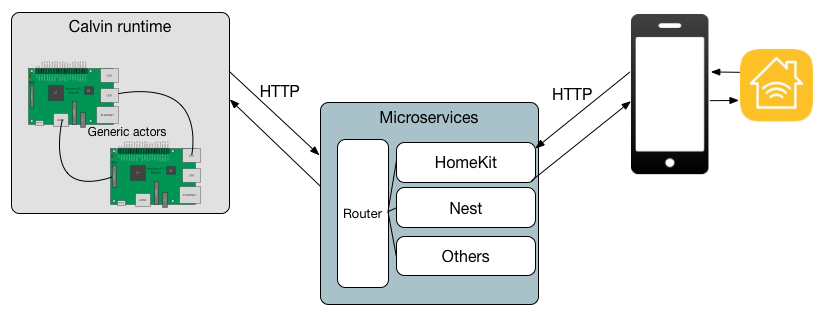
\includegraphics[scale=0.5]{arch2.png}
\end{figure}

Despite the overhead due to the different services, being on the same network, under the
assumption of it being fast enough, the total delay should be more than acceptable.
However the architecture present a weakness,due to the single point-of-failure in the
iOS application, which is the only access to the HomeKit devices.



\subsubsection{Advantages}

Integration with different ecosystems is a new topic, focusing more on the big
picture rather than connecting single devices. Microservices are a bright promise
for the future, for a certain category of problems and integration between ecosystems
fits perfectly into it. There are some pros and cons as there are for any solution,
an example may be the introduced overhead and complexity. Despite the cons the flexibility
introduced my microservices is more valuable, a value for which both overhead and complexity
are paid back.
